\documentclass[12pt, aspectratio=169]{beamer}
 \usepackage{listings}


\usepackage{minted}
 \newminted{python}{bgcolor=gray!25,fontsize=\footnotesize,mathescape}
\usepackage{tikz}
\usetikzlibrary{calc}

\useoutertheme{infolines}

\definecolor{secinhead}{RGB}{249,196,95}
\definecolor{foot}{RGB}{70,67,67}
\definecolor{footfg}{RGB}{198,155,73}
\definecolor{titlebg}{RGB}{51,51,51}

\setbeamercolor{secsubsec}{fg=secinhead,bg=black}
\setbeamercolor{frametitle}{fg=secinhead,bg=titlebg}
\setbeamercolor{footline}{fg=footfg,bg=foot}
\setbeamercolor*{title}{fg=secinhead,bg=titlebg}


% standard enumeration
\setbeamertemplate{enumerate items}{(\arabic{enumi})}

% default itemize
\setbeamertemplate{itemize items}[circle]

% transparency
\setbeamercovered{transparent=9}


\setbeamertemplate{headline}
{
  \leavevmode%
  \hbox{%
  \begin{beamercolorbox}[wd=\paperwidth,ht=4.5ex,dp=3.5ex]{secsubsec}%
    \raggedright
    \hspace*{3em}%
    {\sffamily\small\color{secinhead}\thesection.~\insertsection\hfill\insertsubsection}%
    \hspace*{2em}%
  \end{beamercolorbox}%
  }%
}


\setbeamertemplate{footline}
{%
  \vspace{.1em}
  \leavevmode%
  \hbox{%
  \begin{beamercolorbox}[wd=\paperwidth,ht=1.2ex,dp=0.5ex]{footline}%
    \raggedright
    \hspace*{3em}%
    {\sffamily\scalebox{.7}{\color{secinhead}\insertauthor}\hfill\scalebox{.7}{\inserttitle}\hfill\scalebox{.7}{\insertframenumber/\inserttotalframenumber}}%
    \hspace*{2em}%
  \end{beamercolorbox}%
  }%
}



\setbeamertemplate{frametitle}
{\vskip-2pt
  \leavevmode
  \hbox{%
  \begin{beamercolorbox}[wd=\paperwidth,ht=2.2ex,dp=1ex]{frametitle}%
    \raggedright\hspace*{1.8em}\large\insertframetitle
  \end{beamercolorbox}
  }%
}


\setbeamertemplate{navigation symbols}{}


\graphicspath{
  {img/}
}


\begin{document}
\title{Intro to Programming: With Python}  
\subtitle{(a workshop)}  
\author{Bibek Gautam}
\institute{St. Xavier's College, Maitighar}
\date{\today} 

\begin{frame}[plain]
  \titlepage
\end{frame}
% \begin{frame}[plain]
%   \tableofcontents
% \ end{frame}



\section{Intro to Python} 
\frame{\frametitle{Why Python?} 
  \only<1>{
   \begin{figure}
\hspace{-4em}\centering   
\includegraphics[width=0.28\textwidth]{pythonlogo} 
   \end{figure}
  }
\only<2>{
  \begin{columns}
    \begin{column}{4cm}

   \begin{figure}[left]
   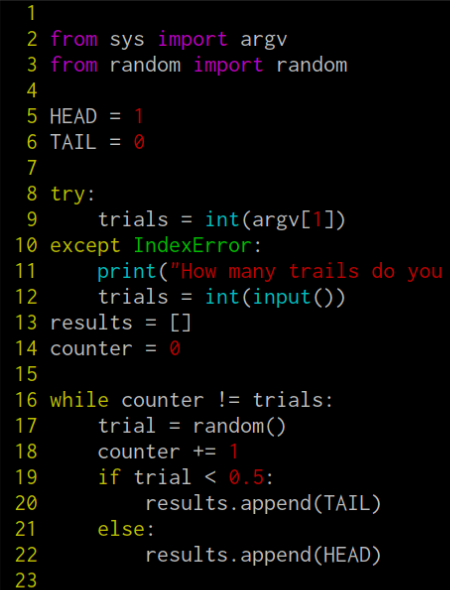
\includegraphics[scale=0.24]{python} 
    \caption{Python}
    \label{fig:py}
  \end{figure}
    \end{column}

    \begin{column}{5cm}
  \begin{figure}[left]
   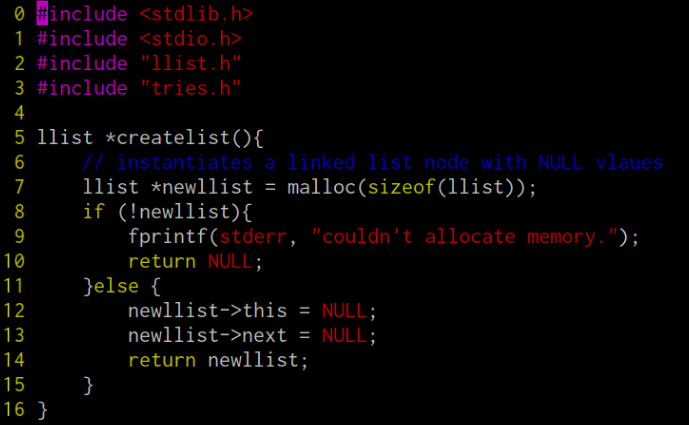
\includegraphics[scale=0.23]{c} 
    \caption{c}
    \label{fig:c}
  \end{figure}
    \end{column}
    
  \end{columns}
}
\only<3>{
  \begin{columns}
    \begin{column}{4cm}
   \begin{figure}
      \hspace{-4em}
   
\includegraphics[width=0.38\textwidth]{youtube}  \\ 
      \vspace{1em}
%\tikz[remember picture, overlay] \node[anchor=center] at ($(current page.center)-(1,1))$) {
\includegraphics[width=0.38\textwidth]{youtube} };
      \hspace{-4em}
   
\includegraphics[width=0.38\textwidth]{mozilla}  \\ 
      \vspace{1em}
      \hspace{-4em}
   
\includegraphics[width=0.38\textwidth]{dropbox} 
   \end{figure}
   \end{column}
    \begin{column}{4cm}
   \begin{figure}
      
\includegraphics[width=0.38\textwidth]{nasa}  \\ 
      \vspace{1em}
      
\includegraphics[width=0.38\textwidth]{bittorrent}  \\ 
      \vspace{1em}
      
\includegraphics[width=0.38\textwidth]{ibm} 
   \end{figure}
   \end{column}
   \end{columns}
 }
\only<4>{
  \begin{columns}
    \begin{column}{4cm}
   \begin{figure}
      \hspace{-4em}
   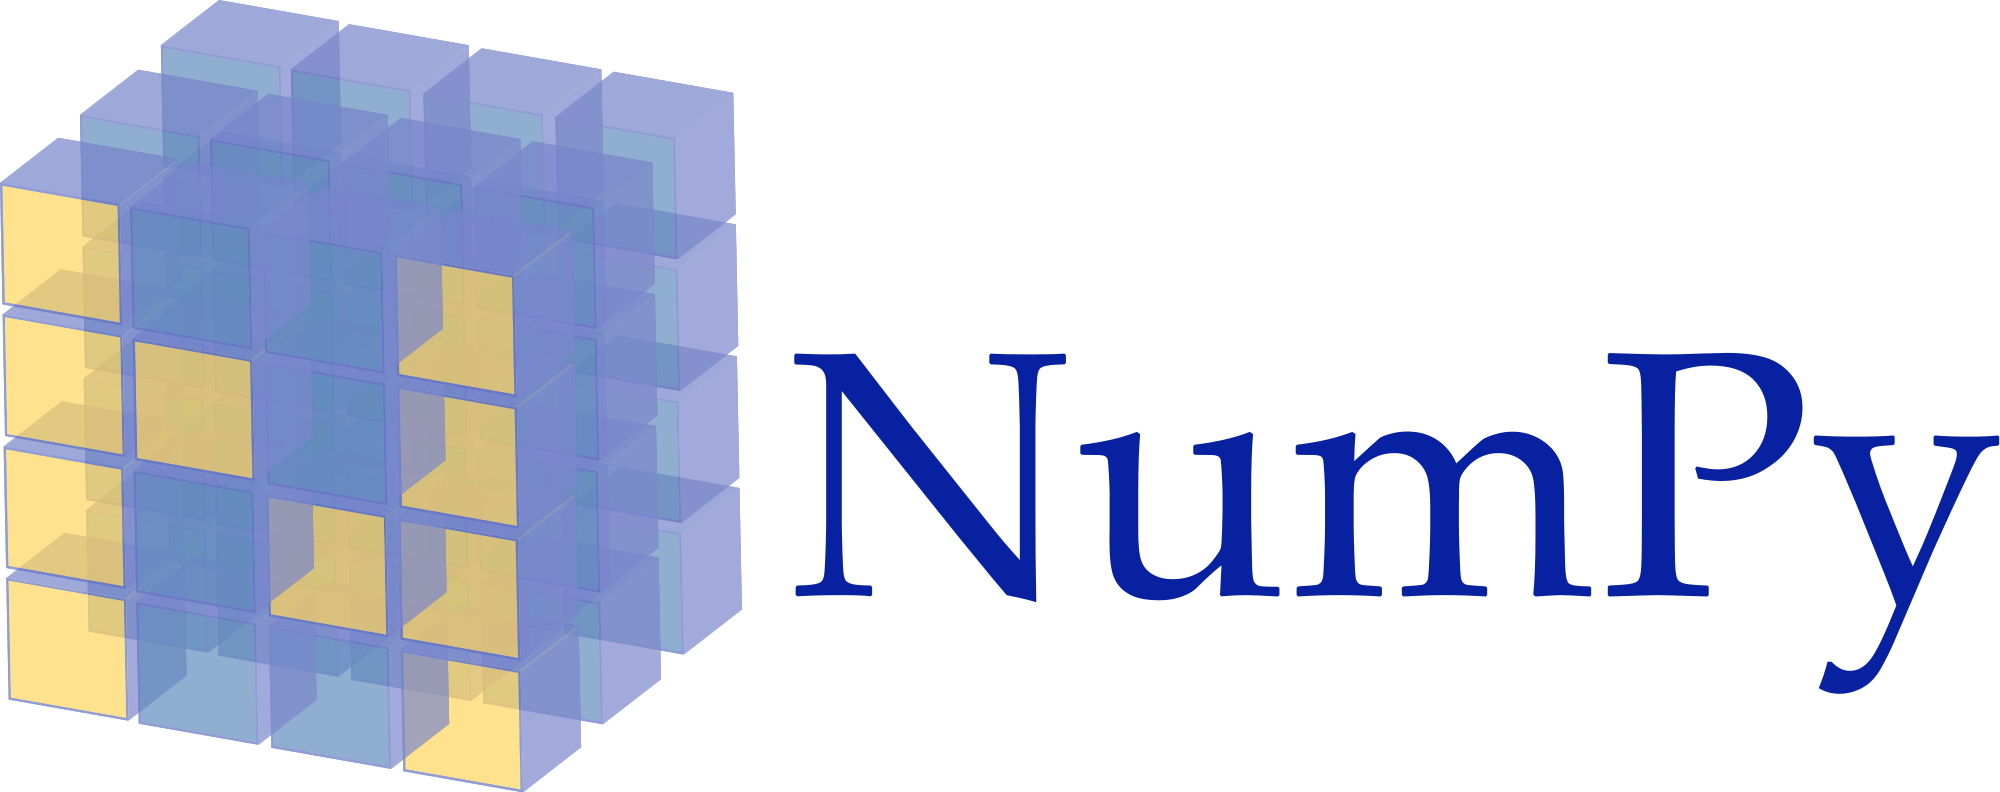
\includegraphics[width=0.38\textwidth]{numpy}  \\ 
      \vspace{1em}
%\tikz[remember picture, overlay] \node[anchor=center] at ($(current page.center)-(1,1))$) {
\includegraphics[width=0.38\textwidth]{youtube} };
      \hspace{-4em}
   
\includegraphics[width=0.38\textwidth]{scipy}  \\ 
      \vspace{1em}
      \hspace{-4em}
   
\includegraphics[width=0.38\textwidth]{tensorflow} 
   \end{figure}
   \end{column}
    \begin{column}{4cm}
   \begin{figure}
      
\includegraphics[width=0.38\textwidth]{matplot}  \\ 
      \vspace{1em}
      
\includegraphics[width=0.38\textwidth]{pandas}  \\ 
      \vspace{1em}
      
\includegraphics[width=0.38\textwidth]{jupyter} 
   \end{figure}
   \end{column}
   \end{columns}
 }
}

\frame{ \frametitle{Compiled Vs. Interpreted}
\begin{figure}
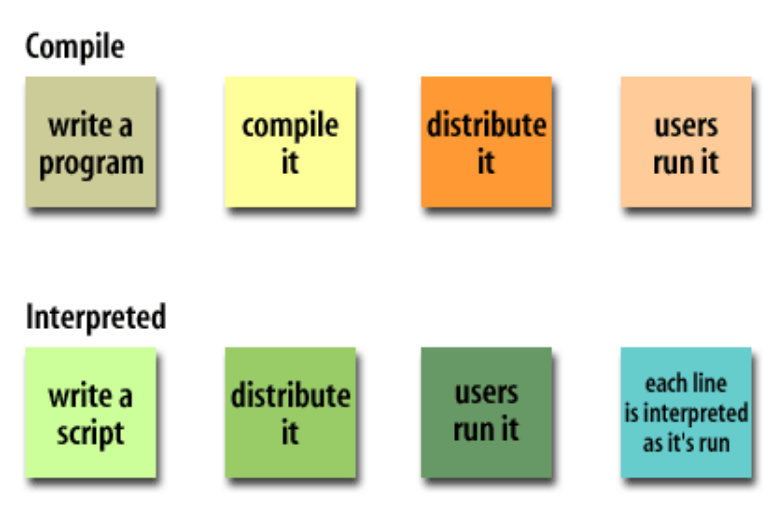
\includegraphics[width=0.5 \textwidth]{cvsi} 
\caption{Compiled Vs. Interpreted}
\end{figure}
}

\section{Setting up Environment}
\subsection{Installing python}
\begin{frame}[fragile]
  \frametitle{On Linux \small{(Ubuntu/Mint or similar)}}
  \begin{minted}{bash}
    $ sudo apt-get update 
    $ sudo apt-get upgrade 
    $ sudo apt-get install spyder python3-matplotlib
    $ sudo apt-get install  python3-scipy python3-pandas
\end{minted}
\end{frame}


\frame{
  \frametitle{On Windows}
  \begin{itemize}
  \item Download and install Anaconda
    \end{itemize}
      \hspace{1em}\textcolor{brown}{ \large{OR}}
      \small
  \begin{itemize}
    \item Download and install Winpython
    \end{itemize}
} 

\section{Python Basics}
\subsection{intro}
\begin{frame}[fragile]
  \frametitle{Hello world and comments}
  \begin{columns}
  \hspace{-2em}\begin{column}{5cm}
  \begin{minted}{python}
  print("Hello World.")

  
  print("Hi")  # this prints "Hi" 

  
  ''' Everything within this is comment.
  This doesn't get evaluated.
  It's all comments!
  '''
  print("hi")
  \end{minted}
  \end{column}
  \begin{column}{5cm}
   \hspace{5em} $\leftarrow$    Hello World \\ 
    \vspace{2em}
    \hspace{5em}$\leftarrow$    inline  \\
    \vspace{3em}
    \hspace{5em}$\leftarrow$    multi-line \\ 
    \vspace{4em}
  \end{column}
 \end{columns}
 
\end{frame}

\begin{frame} [fragile]
  \frametitle{Usual Operations}
  \begin{minted}{python}
   + - * /            # basic arithmetic 
   //                 # integer division
   ++ --              # increment
   += -+ *=           # 
   **                 # power
   ==  != <= >= < >   # comparision
 \end{minted}
\vspace{2em}
\emph{Order of Operation matters!}
\end{frame}

\subsection{Data types}
\begin{frame} [fragile]
  \frametitle{Variables \& Data types}
\begin{minted}{python3}
     age = 5               # integer
     height = 123.2        # float
     college = "SXC"       # string
     isAlumni = True       # boolean
     favNum = 2 + 3j       # complex number

     # and a few more

\end{minted}
\end{frame}

\begin{frame}[fragile]
  \frametitle{Strings}
\begin{minted}{python3}
   name = "John Doe"
   sentence = "My name is " + name +"."

   print(sentence, end=".")

   multiLine = ''' This is a
   string with multiple
   lines in it '''
\end{minted}
  \pause
  \textcolor{brown}{How would you print :  He said "I'm Lucky" ?} 
  \pause
  \begin{minted}{python3}
   print("He said \"I'm Lucky\"")  
   ''' \ is a way to escape special meaning (aka
      escape sequence) '''
\end{minted}
  \vspace{.5em}
\end{frame}

\begin{frame}[fragile]
  \frametitle{Strings}
\textbf{Some useful string methods: }
\begin{minted}{python3}
     .split()
     .replace("," , ".")
     .find()
     .count()
     .isalnum()
     .int()
     .isalpha()
     .isdigit()
     .strip()
     
\end{minted}
\end{frame}


\subsubsection{inputs}
\begin{frame}[fragile]
  \frametitle{Taking inputs: }
\textbf{As simple as it gets...} \\
\vspace{1em}
\begin{minted}{python3}
    age = input("Enter your age: ")
    print("You've lived for about", int(age)*365, "days!")
\end{minted}
\vspace{2em}\pause
\textbf{What if i enter characters and not digits?}
\vspace{2em}

\end{frame}

\subsubsection{inputs}
\begin{frame}[fragile]
  \frametitle{Practice}
     \textbf{   Here is a problem for you to try: }\\ 
    \vspace{1em}
Get input from user and print it out by splitting it at space character.
\end{frame}




\subsubsection{lists}
\begin{frame}[fragile]
  \frametitle{Lists}
  \begin{itemize}
  \item collection of items
  \item could be heterogenous
  \item mutable
  \end{itemize}
  \vspace{2em}
\begin{minted}{python3}
shopping_list = ['tomatoes', 'potatoes', 'apples', 'juice', 'guava']

print("First item:", shopping_list[0])
\end{minted}
\end{frame}

\begin{frame}[fragile]
  \frametitle{Lists}
\textbf{List indexing and splicing}
\vspace{2em}
\begin{minted}{python3}

 list[1:3]    # from index 1 to 3 (excluding 3)

 list[:3]     # splicing
 list[2:]

 new_list = list[:]  # makes a copy
 list_2 = list       # giving another name

\end{minted}
\end{frame}

\begin{frame}[fragile]
  \frametitle{Lists}
\textbf{List inside of list}
\begin{minted}{python3}
matrix = [[1,2,3], [4,5,6], [7,8,9]]

print(matrix[1][0])       # this prints 6 !

matrix.append([10,11,12]) # now matrix is 4*3

matrix.insert(2,[2, 2, 3])  # inserts new row at index 2

a = [1, 4, 5]  
matrix = matrix + a         # combining to lists.
\end{minted}
\end{frame}

\begin{frame}[fragile]
  \frametitle{Lists}
\textbf{Some list useful methods: }
\begin{minted}{python3}
list.sort()
list.reverse()  # sorting

sorted()    # returns an iterable of sorted items

del(list[4])     # delete item at index 4
max() and min()  # first and last for non numbers)
\end{minted}
\end{frame}

\begin{frame}[fragile]
  \frametitle{Lists}
\textbf{Some \textit{more} list useful methods: }
\vspace{1em}
\begin{minted}{python3}
list = [3,1,4] 
len(list)      # length of the list (returns 3)

a = 3 in list  # a is True now
# item in list   evaluates to either true or false.

.find()
.search()
.replace()

\end{minted}
\end{frame}

\begin{frame}[fragile]
  \frametitle{Lists}
\vspace{1em}
\textbf{string are almost like lists !}
\end{frame}

\subsubsection{Tuple}
\begin{frame}[fragile]
  \frametitle{Tuples}
\textbf{What are tuples?}
\begin{itemize}
\item list that cant be changed. 
\item fixed length, can't be appended or deleted.
\item comparable to struct in C
\item takes less memory and is faster 
\item list() and tuple() function to go back and forth between lists and tuple
\end{itemize}
\pause
\begin{minted}{python3}
point = (x, y)
student = (name, roll, enrollYr)

# they can be sliced just like lists
student[0]  # gives name of student
point[1]    # gives y co-ordinate of point

\end{minted}
\end{frame}

\subsubsection{Dictionary}
\begin{frame} [fragile]
  \frametitle{Dictionary}
  \begin{itemize}
  \item Dictionary stores key-value pair data \pause
  \item  also known as hash table, look-up table in other languages \pause
  \end{itemize}
  \vspace{1em}
\begin{minted}{python3}
        >>> 
        >>> capitals = {"Nepal": "Kathmandu",
                        "India": "New Delhi",
                        "Pakistan": "Islamabad"}

        >>> capital["Pakistan"]       # returns Islamabad
        >>> capital["France"] = "Rome"
        >>> del(capital["France"])    # as you'd expect
\end{minted}
\end{frame}

\begin{frame} [fragile]
  \frametitle{Dictionary}
\textbf{Some dictionary methods: }
 \begin{minted}{python3}
        >>> len(dict)
        >>> dict.keys()
        >>> dict.values()
 \end{minted}
\vfill
\end{frame}

\subsection{Conditionals}
\begin{frame} [fragile]
  \frametitle{Conditionals - if/else}
\textbf{When your code requires decision making based on conditions}
\vspace{1em}
 \begin{minted}{python3}

     >>> if age > 16:
     ...    print("You're old enough to drive")
     ... elif age > 25:
     ...    print("You're old enough to get married")
     ... else:
     ...     print("You're not old enough to drive or get married.")
 
\end{minted}
\vspace{1em}
\textbf{Python also has keywords like: and, or, not, True, False}
\vspace{1em}
\end{frame}


\subsection{Loops}
\frame{\frametitle{Loops}
  \only<1>{
    \centering
  \begin{itemize}
  \item loops are for when you have to execute a block of code multiple times.
  \item there are two modes of loops: \textbf{for} and \textbf{while} loop. 
  \end{itemize}
  }
  \only<2>{
  \begin{figure}
    \centering
   \includegraphics[scale=0.34]{loop} 
    \caption{Basic Logic of Loop }
    \label{fig:loop}
  \end{figure}
  }
}
\frame{\frametitle{For loop}
  \begin{itemize}
  \item For loop iterates through a collection of iterables object or\\
    generator function \pause
  \item for eg. a list is an iterable and so is a string \pause
  \item dictionary is also an iterable \pause
  \end{itemize}
\vspace{2em}
 \textbf{What are generator functions?} \\ 
  \begin{itemize}
    \item range() is an example
    \item another is open()  which is used to open files. \textit{We'll come to this later.} 
  \end{itemize}
}

\frame{\frametitle{For loop}
\only<1->{
 \textbf{Let's talk about range() } \\ 
 \begin{figure}
   \includegraphics[scale=0.50]{forloop} 
   \caption{for loop with range}
 \end{figure}
}

\only<2>{
\textcolor{gray}{ range(s, e, stp) with start, end, and step} 
  }
}

\begin{frame}[fragile]
  \frametitle{Loops}
 \textbf{Some more range: } 
% wont give you use \only with minted and (arg, arg) sort of thing inside. fckn stupid
\begin{minted}{python3}
  for i in range(1,11): 
      print i
  for i in range(1,21,2): 
      print i
  for i in range(11, 1, -1):  # doesn't include i 
      print i
\end{minted}
 \end{frame}

\begin{frame}[fragile]
  \frametitle{Loops}
 \textbf{Looping through lists} 
\begin{minted}{python3}
        for item in list:
            print(item)
\end{minted}
 \vspace{4em}
 \pause
\textbf{But, what if you have multiple dimensional array ??\\ }
 \pause
 \vspace{2em}
\textcolor{gray}{\textbf{That's when you need nested loops !}}
 \end{frame}


\begin{frame}[fragile]
  \frametitle{Nesting Loops}
 \textbf{Nesting means using loops inside of loops : } 
 \vspace{2em}
\begin{minted}{python3}
  list_of_lists = [ [1,2,3], [4,5,6], [7,8,9] ] 
  for list in list_of_lists:
      for item in list:
          print(item)

  # above prints 1 through 9 when done

\end{minted}
 \end{frame}
 
 \begin{frame}
   \frametitle{While loop}
   \textbf{When you want to do something \\ 
     \textit{untill} a certain condition is
  \textit{true} use \textit{while} loops}
  \vspace{2em}
   \begin{itemize}
   \item Use while loop when you dont have a tidy data structure to iterate through
   \item or don't have a relevant generator function.
   \item when you want to decide when to stop from within the loop \pause
   \item  Let's see what I mean!
   \end{itemize}
  \vspace{4em}
 \end{frame}


 \begin{frame}[fragile]
   \frametitle{While loop}
   \textbf{ How many perfect cube numbers are less than 100000?}
   \vspace{2em} \pause
\begin{minted}{python3}
   this_many = 0      # this counts the number of cube numbers found 
   cuberoot = 1
   while cuberoot**3 < 100000:
       this_many += 1
       cuberoot += 1

   print(this_many)   # executes when the loop completes.
\end{minted}
 \end{frame}

 \subsection{Functions}
 \begin{frame}[fragile]
   \frametitle{Functions}
\textbf{About functions:}
   \begin{itemize}
   \item Functions are similar to what we understand from maths.
   \pause
   \item Functions take some input(s) and return some ouput(s)
   \pause
   \item input and output could be different type of data
   \end{itemize}
   \pause
\textbf{Why use functions?}
   \pause
\begin{itemize}
   \item Functions allow us to divide the problem into logical chunks of
     sub-problems that we can separately deal with.
   \pause
   \item makes code more readable and more structured!
   \pause
   \item makes debugging easy !
\end{itemize}
\end{frame}


 \begin{frame}[fragile,fragile]
   \frametitle{Functions}
\textbf{Let's see an example}
\vspace{2em}
\begin{minted}{python3}
    def toPercent(num, denum):
        ''' Takes a fraction and returns 
        equivalent percentage '''
        percent = num/denum  * 100
        percent = int(percent)  
        return percent      # return is used to output

    print("4/5 = ", toPercent(4,5), "%.")

\end{minted}
 \end{frame}


 \begin{frame}[fragile]
   \frametitle{Namescope}
   \begin{itemize}
   \item Namescope is like a dictionary that maps variable \\
     names to their values 
   \item Every function has its own namespace.
   \item which means variable declared in one function \\
     can't be accessed from another.
   \end{itemize}
 \end{frame}

\section{Object Oriented Programming with Python}
\vspace{2em}
 \begin{frame}[fragile]
   \frametitle{Overview OOP}
   \begin{figure}
     \centering
   \includegraphics[width=0.5\textwidth]{minimilitia}  
     \caption{OOP in Games}
   \end{figure}
 \end{frame}


 \begin{frame}[fragile]
   \frametitle{Objects heirarchy}
  \begin{figure}
     \centering
     \includegraphics[width=0.25\textwidth]{objects}  
     \caption{Objects and inheritence}
   \end{figure}

 \end{frame}


 \begin{frame}[fragile]
   \frametitle{Objects heirarchy}
  \textbf{Attributes and methods} \\ 
  Variables \textit{encapculated} inside a class are its attributes. And functions
  \textit{encapculated} within a class are called its methods.
  \linebreak
  \linebreak
  \textbf{Parent Class} \\ 
  The class above a class in class heirarchy is called its parent.
  \linebreak
  \linebreak
  \textbf{Child class} \\ 
  The classes that derive from a class are its children.
  \linebreak
  \linebreak
  \textbf{Inheritence} \\
\small{  Child class retains all the methods and attributes from the parents. This is}
  known as inheritence.
 \end{frame}


 \begin{frame}[fragile]
   \frametitle{To be continued...}
   \begin{figure}
     \vspace{-2em}
   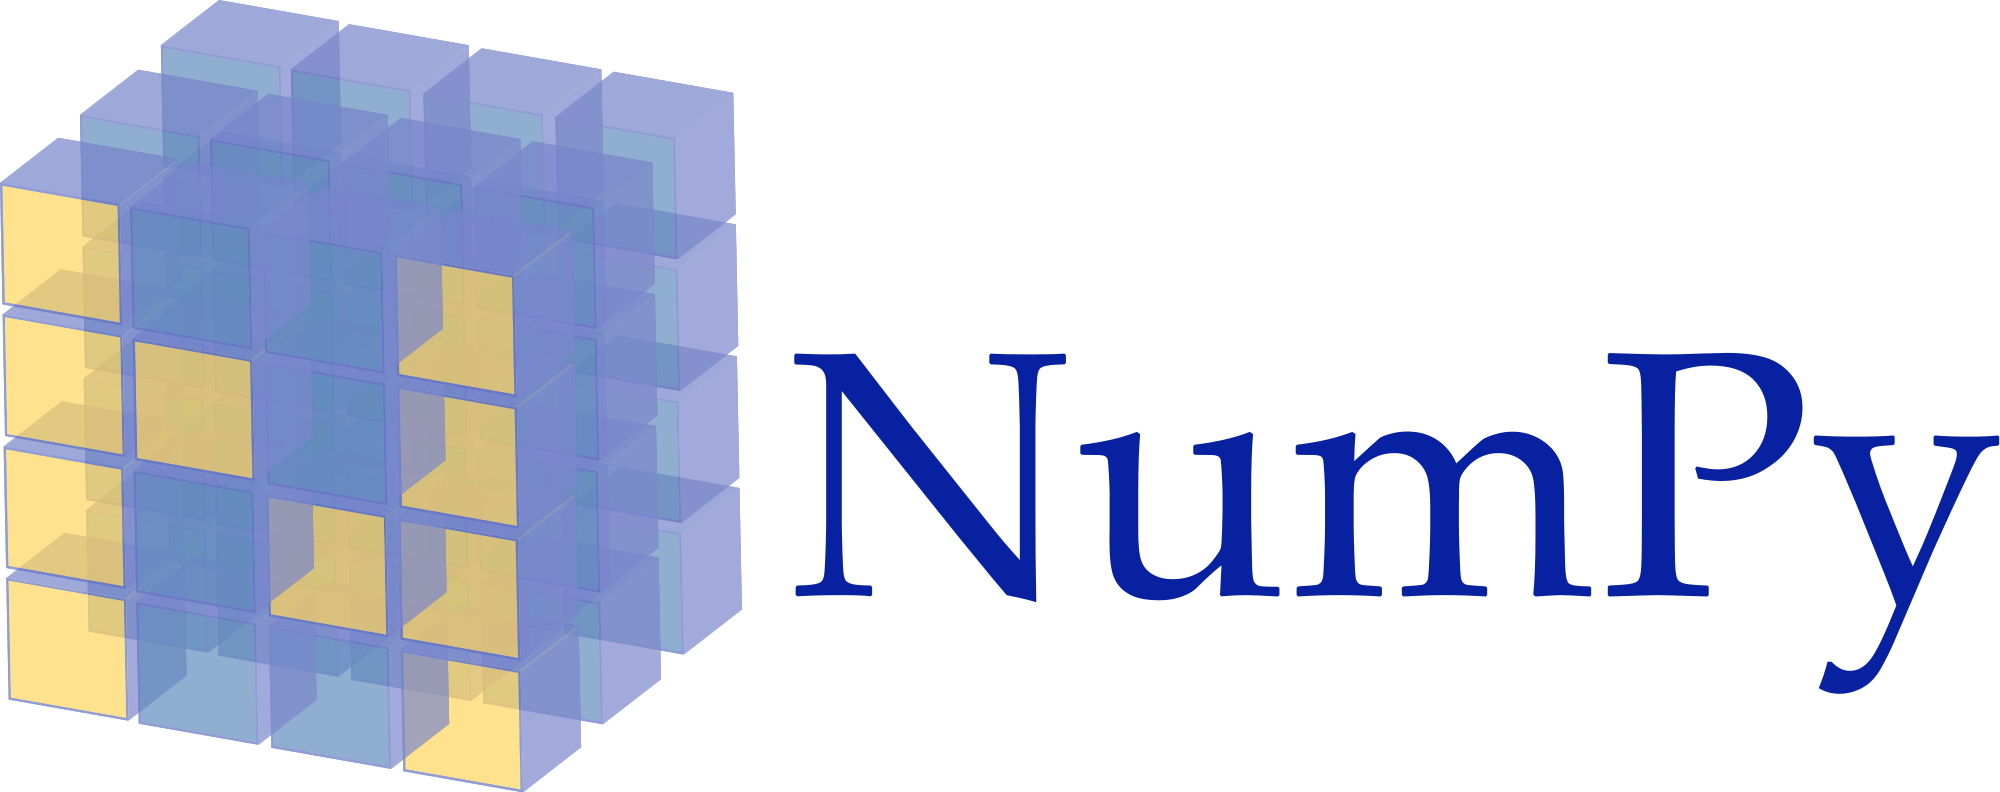
\includegraphics[width=0.20\textwidth]{numpy}   
   
\includegraphics[width=0.08\textwidth]{scipy}  \\ 
   
\includegraphics[width=0.24\textwidth]{matplot} 
   \end{figure}


   \hspace{12em}\centering\colorbox{gray}{\textbf{ \linebreak\huge{Thank You!}\linebreak}}
 \end{frame}

 \end{document}